%20 min preso!
\documentclass[aspectratio=169,xcolor=table,english]{beamer}
\usepackage{beamerthemesplit}
\usepackage{wrapfig}
\usetheme{SPbGU}
\usepackage{pdfpages}
\usepackage{amsmath}
\usepackage{mathtools}
\usepackage{cmap}
\usepackage{subcaption}
\usepackage[utf8]{inputenc}
\usepackage[T1, T2A]{fontenc}
\usepackage[]{babel}
\usepackage{indentfirst}
\usepackage{amsmath}
\usepackage{tikz}
\usepackage{multirow}
\usepackage[noend]{algpseudocode}
\usepackage{algorithm}
\usepackage{algorithmicx}
\usepackage{fancyvrb}
\usetikzlibrary{calc}
\usetikzlibrary{shapes,arrows}
\usetikzlibrary{arrows,automata}
\usetikzlibrary{positioning}
\usetikzlibrary{fit}

\usepackage{kbordermatrix} % include package @ document preamble
\renewcommand{\kbldelim}{(} % change default array delimiters to parentheses
\renewcommand{\kbrdelim}{)}

\newcommand\mca{\multicolumn{1}{c}{\cellcolor{red}\textbf{\{a\}}}}
\newcommand\mcb{\multicolumn{1}{c}{\cellcolor{red}\textbf{\{b\}}}}

\usepackage{tabularx}
\newcolumntype{Y}{>{\raggedleft\arraybackslash}X}

\renewcommand{\thealgorithm}{}

\newtheorem{mytheorem}{Theorem}
\renewcommand{\thealgorithm}{}

\newcommand{\tikzmark}[1]{\tikz[overlay,remember picture] \node (#1) {};}
\def\Put(#1,#2)#3{\leavevmode\makebox(0,0){\put(#1,#2){#3}}}

\newcommand{\ltz}{$< 1$}

\tikzset{
    state/.style={
           rectangle,
           rounded corners,
           draw=black, very thick,
           minimum height=2em,
           inner sep=2pt,
           text centered,
           },
}

\beamertemplatenavigationsymbolsempty

\title[DPLL \& CDCL]{Структуры данных в алгоритмах DPLL и CDCL}
% \subtitle[YaccConstructor]{Parsing techniques for graph analysis}
% То, что в квадратных скобках, отображается в левом нижнем углу.
\institute[СПбГУ]{
Санкт-Петербургский Государственный университет
}

% То, что в квадратных скобках, отображается в левом нижнем углу (прикольно).
\author[Егор Орачев]{\textbf{Егор Орачев}}
\date{13 декабря, 2021}

\begin{document}
{
\begin{frame}[fragile]
  \begin{table}
  \centering
  \begin{tabularx}{\linewidth}{YcX}
     \begin{minipage}[t]{0.7\textwidth}\center \vspace{-1cm} 
     Дополнительные главы матлогики
      \end{minipage}
    & \hfill 
\includegraphics[height=2.0cm]{pictures/SPbGU_Logo.png}
  \end{tabularx}
  \end{table}
  \titlepage
\end{frame}
}

\begin{frame}[fragile] \frametitle{Терминология}
    \begin{itemize}
        \item \textbf{Объекты}
        \begin{itemize}
            \item Переменная $x$
            \item Литерал $l$ это либо переменная $x$, либо ее отрицание $\overline{x}$
            \item Кляуза (англ. clause) это конечное множество литералов $\omega = \{l_1, ..., l_n\}$
            \item Формула это конечное множество кляуз $\phi = \{ \omega_1, ..., \omega_m\}$
        \end{itemize}
        \item \textbf{Интерпретация}
        \begin{itemize}
            \item Присвоенное переменной значение $\upsilon(x) \in \{0,~1\}$, $\upsilon(\overline{x})=1-\upsilon(x)$
            \item Кляуза $\omega = \{l_1, ..., l_n\}$ выполнена, если хотя бы для одного литерала $\upsilon(l_i)=1$
            \item Формула $\phi = \{ \omega_1, ..., \omega_m\}$ выполнена, если все $\omega_i$ выполнены для $\upsilon$
        \end{itemize}
    \end{itemize}
\end{frame}

\begin{frame}[fragile] \frametitle{Алгоритм}
    \begin{minipage}[m]{0.5\linewidth}
    \begin{enumerate}
        \item Поиск поиск переменной для присваивания (\textbf{decision process}).
        \item Получение логических следсвий из присваивания (\textbf{implication process})
        \item Отмена присвиваний и откат к раннему состоянию (\textbf{backtracking process}).
    \end{enumerate}
    \end{minipage}\hfill
    \begin{minipage}[m]{0.5\linewidth}
        \begin{figure}
            \centering
            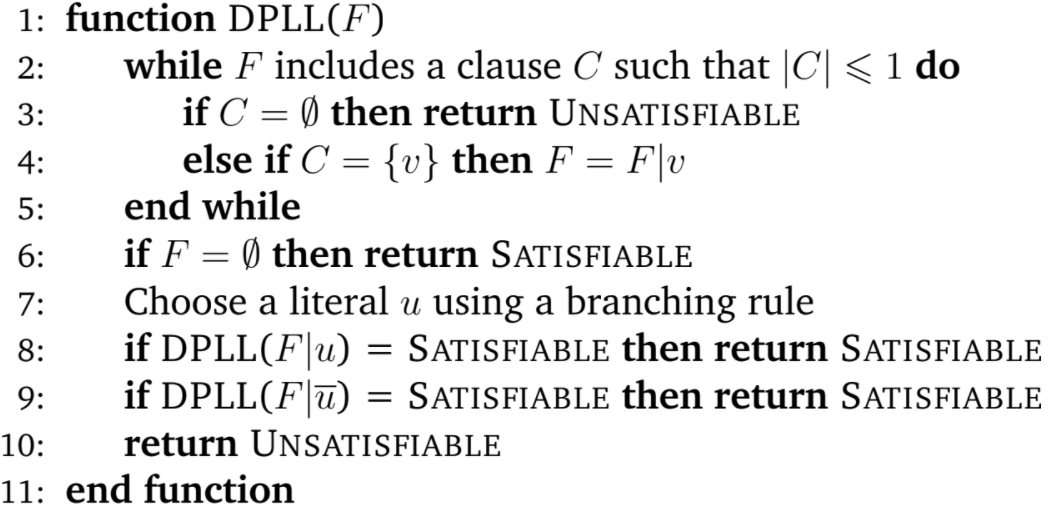
\includegraphics[width=0.9\textwidth]{figures/dpll.png}
            \caption{Общая структура dpll алгоритма (изображение из работы [6])}
        \end{figure}
    \end{minipage}
\end{frame}

\begin{frame}[fragile] \frametitle{Проблемы}
    \begin{itemize}
        \item Как эффективно удалять кляузы?
        \item Как эффективно искать \textit{unit}-кляузы?
        \item Как эффективно удалять литералы из кляуз? 
        \item Как эффективно откатывать изменения?
        \item Как эффективно хранить граф импликаций?
        \item ...
    \end{itemize}
\end{frame}

\begin{frame}[fragile] \frametitle{Структура презентации}
    \begin{enumerate}
        \item Adjacency lists
        \begin{enumerate}
            \item Assigned literal hiding
            \item The counter-based approach
            \item Counter-based with satisfied
            \item Satisfied clause and assigned literal hiding
        \end{enumerate}
        \item Lazy data structures
        \begin{enumerate}
            \item Sato’s head/tail lists
            \item Chaff ’s watched literals
            \item Head/tail lists with literal sifting
            \item Watched literals with literal sifting
        \end{enumerate}
        \item Tries
        \item Детали реализации
    \end{enumerate}
\end{frame}

\begin{frame}[fragile] \frametitle{1. Adjacency lists}
    \begin{minipage}[m]{0.5\linewidth}
        \begin{itemize}
            \item Каждая кляуза хранит список литералов, которые в нее входят
            \item Каждый литерал хранит список кляуз, в которых он встречается
            \item \textit{Adjacency} т.е. литералы и кляузы смежны (что достигается засчет списков)
            \item В общем случает \textit{adjacency list} --- когда литерал имеет \textbf{полный} список кляуз, в которые он входит
        \end{itemize}
    \end{minipage}\hfill
    \begin{minipage}[m]{0.45\linewidth}
        \begin{figure}
            \centering
            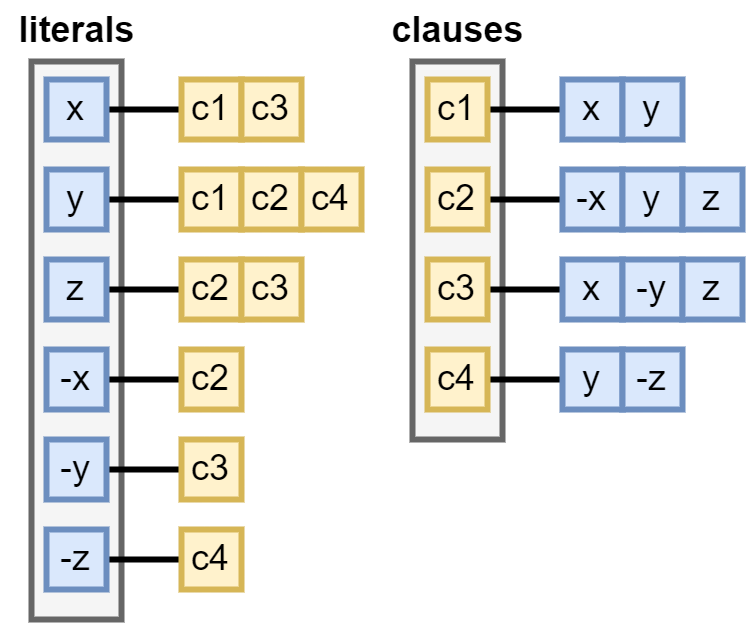
\includegraphics[width=0.8\textwidth]{figures/adjacency lists.png}
            \caption{Списки смежности для формулы $\{x,y\},\{\overline{x},y,z\},\{x,\overline{y},z\},\{y,\overline{z}\}$}
        \end{figure}
    \end{minipage}
\end{frame}

\begin{frame}[fragile] \frametitle{1.1 Assigned literal hiding}
    \begin{minipage}[m]{0.5\linewidth}
        \begin{itemize}
            \item \textbf{Идея}: разделить литералы внутри кляузы на отлельные списки
            \item При присваивании значения литералу, перемещать его в соответсвующий списов
            \item \textbf{Backtracking}: необходимо применить операции в обратном порядке
            \item \textit{На практике всегда уступает отсальным структурам, поэтому в явном виде не используется}
        \end{itemize}
    \end{minipage}\hfill
    \begin{minipage}[m]{0.45\linewidth}
        \begin{figure}
            \centering
            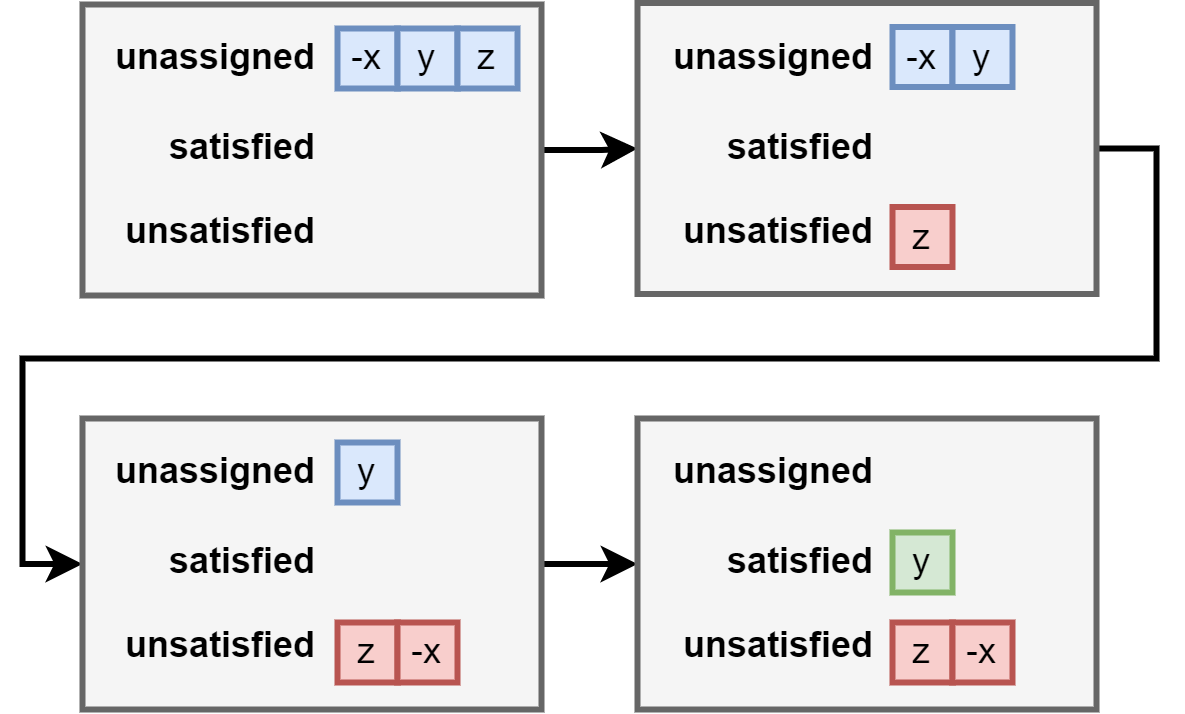
\includegraphics[width=0.85\textwidth]{figures/assigned lit hiding.png}
            \caption{Пример использования для $\{\overline{x},y,z\}$, последовательность присваиваний $z \rightarrow 0$, $\overline{x} \rightarrow 0$, $y \rightarrow 1$}
        \end{figure}
    \end{minipage}
\end{frame}

\begin{frame}[fragile] \frametitle{1.2 The counter-based approach}
    \begin{minipage}[m]{0.5\linewidth}
        \begin{itemize}
            \item \textbf{Идея}: вести только подсчет литералов каждого вида внутри кляузы
            \item Завести три счетчика: \textbf{total}, \textbf{satisfied}, \textbf{unsatisfied}
            \item Обновлять счетчики, когда литералу присвоено значение
            \item Необходимо итерироваться по всему списку литералов, чтобы найти \textit{unit-литерал}
            \item \textbf{Backtracking}: необходимо вернуть счетчики в изначальное состояние
            \item \textbf{Применение}: GRASP
        \end{itemize}
    \end{minipage}\hfill
    \begin{minipage}[m]{0.45\linewidth}
        \begin{figure}
            \centering
            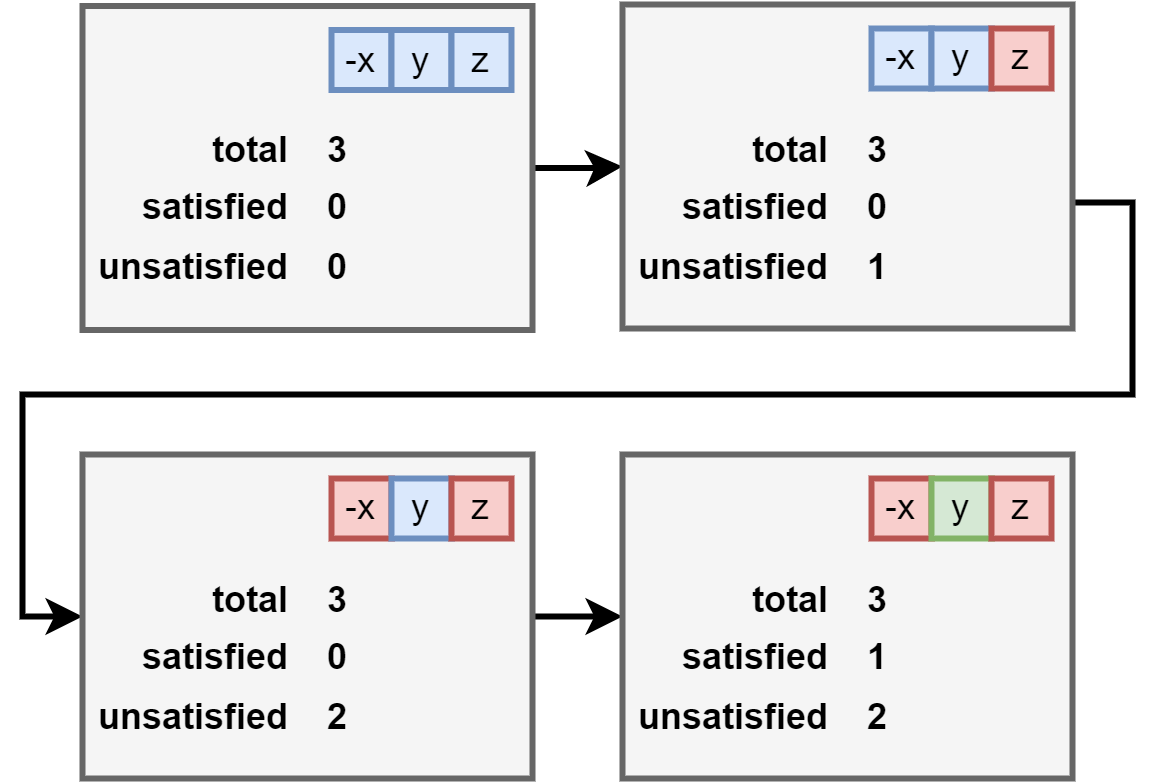
\includegraphics[width=0.85\textwidth]{figures/counter based.png}
            \caption{Пример использования для $\{\overline{x},y,z\}$, последовательность присваиваний $z \rightarrow 0$, $\overline{x} \rightarrow 0$, $y \rightarrow 1$}
        \end{figure}
    \end{minipage}
\end{frame}

\begin{frame}[fragile] \frametitle{1.3 Counter-based with satisfied clause hiding}
    \begin{itemize}
        \item \textbf{Проблема}: список кляуз большой (и может расти)
        \item \textbf{Мотивация}: при очерендном присваивании литералу значения интересуют только невыполненные еще кляузы
        \item \textbf{Идея:} удалять (прятать) выпленную кляузу из спиков всех литералов
        \item \textbf{Backtracking}: необходимо восстановить списки
        \item \textbf{Применение}: Scherzo covering problem
        \item \textit{На практике недостаточно эффективно в сравнении с простым counter-based подходом} 
    \end{itemize}
\end{frame}

\begin{frame}[fragile] \frametitle{1.4 Satisfied clause and assigned literal hiding}
    \begin{itemize}
        \item \textbf{Проблема}: поиск unit-литерала
        \item \textbf{Мотивация}: при очерендном присваивании литералу значения хотим найти новый unit-литерал в кляузах
        \item \textbf{Идея:} удалять (прятать) невыполненные литералы внутри кляузы
        \item \textbf{Backtracking}: необходимо восстановить литералы
        \item \textit{На практике недостаточно эффективно в сравнении с простым counter-based подходом} 
    \end{itemize}
\end{frame}

\begin{frame}[fragile] \frametitle{2. Lazy data structures}
    \begin{minipage}[m]{0.5\linewidth}
        \begin{itemize}
            \item \textbf{Проблема}: список кляуз большой (и может расти)
            \item \textbf{Идея}: когда литералу присвоено значение, не во всех кляузах происходит что-то \textit{интересное}
            \item Каждая кляуза хранит список литералов, которые в нее входят
            \item Каждый литерал хранит \textbf{сокращенный} список кляуз, в которых он встречается
            \item В общем случает \textit{lazy data structures} --- когда литерал имеет \textbf{сокращенный} список кляуз
        \end{itemize}
    \end{minipage}\hfill
    \begin{minipage}[m]{0.45\linewidth}
        \begin{figure}
            \centering
            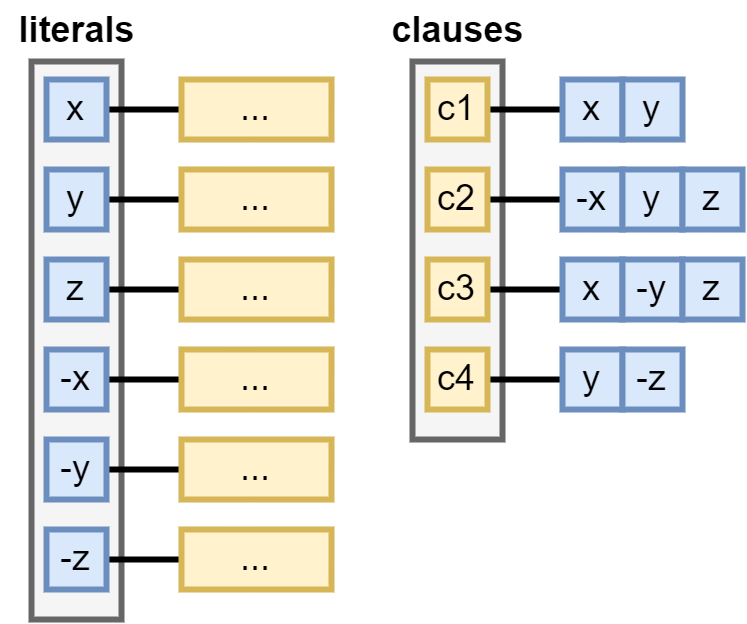
\includegraphics[width=0.8\textwidth]{figures/lazy data structure.png}
            \caption{Представление формулы  $\{x,y\},\{\overline{x},y,z\},\{x,\overline{y},z\},\{y,\overline{z}\}$}
        \end{figure}
    \end{minipage}
\end{frame}

\begin{frame}[fragile] \frametitle{2.1 Sato’s head/tail lists}
    \begin{minipage}[m]{0.55\linewidth}
        \begin{itemize}
            \item Два указателя внутри каждой кляузы: \textit{head (H)} и \textit{tail (T)}, изначально указывают на начало и конец кляузы соответсвенно
            \item У каждого литера есть два списка кляуз: где он \textit{head} и \textit{tail} соответсвенно
            \item Каждый раз, когда литералу присвоено значение, новые \textit{head} или \textit{tail} необходимо найти
            \item \textbf{Backtracking}: необходимо восстановить все указатели
            \item \textbf{Применение}: SATO SAT solver
        \end{itemize}
    \end{minipage}\hfill
    \begin{minipage}[m]{0.4\linewidth}
        \begin{figure}
            \centering
            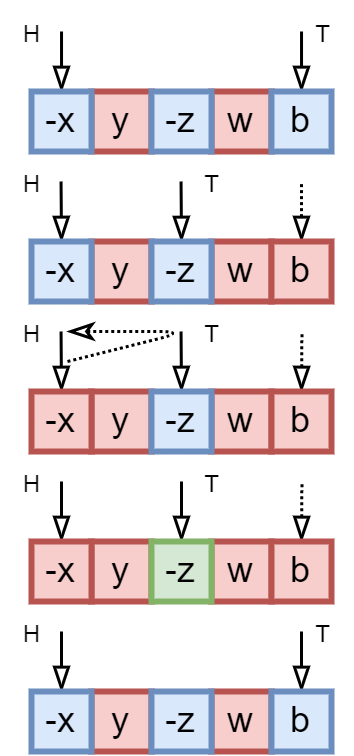
\includegraphics[width=0.4\textwidth]{figures/head tail.png}
            \caption{Пример использования для $\{\overline{x},y,\overline{z},w,b\}$, последовательность присваиваний $y \rightarrow 0$, $w \rightarrow 0$, $b \rightarrow 0$, $\overline{x} \rightarrow 0$, $\overline{z} \rightarrow 1$}
        \end{figure}
    \end{minipage}
\end{frame}

\begin{frame}[fragile] \frametitle{2.2 Chaff ’s watched literals}
    \begin{minipage}[m]{0.55\linewidth}
        \begin{itemize}
            \item \textbf{Идея}: важные состояния - 0 свободных литералов, 1 или много
            \item Два указателя в каждой кляузе на литерал
            \item У каждого литера есть список кляуз, где он \textit{watched}
            \item Каждый раз, когда литералу присвоено значение, новый \textit{watched}-литерал необходимо найти
            \item \textbf{Backtracking}: ничего не надо делать
            \item \textbf{Применение}: Chaff \& MiniSat
        \end{itemize}
    \end{minipage}\hfill
    \begin{minipage}[m]{0.4\linewidth}
        \begin{figure}
            \centering
            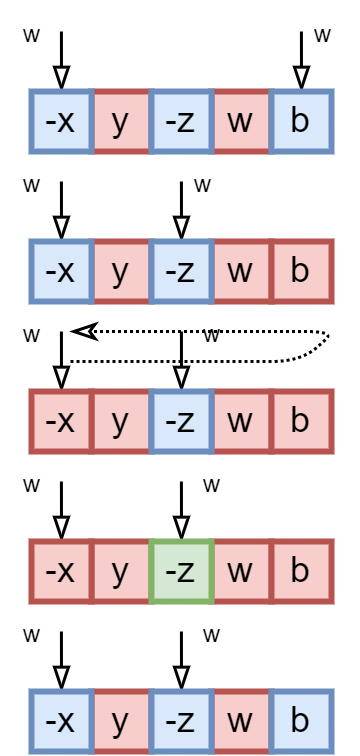
\includegraphics[width=0.4\textwidth]{figures/watched literals.png}
            \caption{Пример использования для $\{\overline{x},y,\overline{z},w,b\}$, последовательность присваиваний $y \rightarrow 0$, $w \rightarrow 0$, $b \rightarrow 0$, $\overline{x} \rightarrow 0$, $\overline{z} \rightarrow 1$}
        \end{figure}
    \end{minipage}
\end{frame}

\begin{frame}[fragile] \frametitle{2.3 Head/tail lists with literal sifting}
    \begin{minipage}[m]{0.55\linewidth}
        \begin{itemize}
            \item \textbf{Проблема}: проблематично откатывать изменения
            \item \textbf{Идея}: переупорядочивать литералы в соответсвии с уровнем дерева решения
            \item Требуются всего 4 указателя на литералы внутри кляузы 
            \item \textit{sifting} - просеивание
            \item \textbf{Backtracking}: отодвинуть \textit{head/tail} указатели влево/вправо соответсвенно 
        \end{itemize}
    \end{minipage}\hfill
    \begin{minipage}[m]{0.4\linewidth}
        \begin{figure}
            \centering
            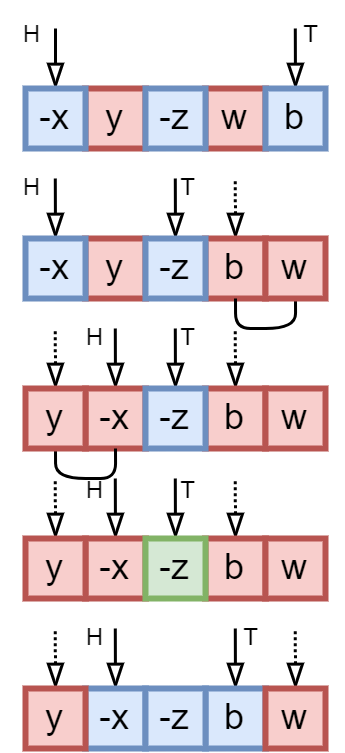
\includegraphics[width=0.4\textwidth]{figures/head tail sifting.png}
            \caption{Пример использования для $\{\overline{x},y,\overline{z},w,b\}$, последовательность присваиваний $y \rightarrow 0$, $w \rightarrow 0$, $b \rightarrow 0$, $\overline{x} \rightarrow 0$, $\overline{z} \rightarrow 1$}
        \end{figure}
    \end{minipage}
\end{frame}

\begin{frame}[fragile] \frametitle{2.4 Watched literals with literal sifting}
    \begin{minipage}[m]{0.55\linewidth}
        \begin{itemize}
            \item \textbf{Проблема}: необходимо итерироваться по всем литералам
            \item \textbf{Идея}: переупорядочивать литералы в соответсвии с уровнем дерева решения
            \item Требуются всего 4 указателя на литералы внутри кляузы
            \item Когда литералу присвоено значение, надо двигать указатель только в пределах неотсортированных регионов
            \item \textbf{Backtracking}: ничего не надо делать
        \end{itemize}
    \end{minipage}\hfill
    \begin{minipage}[m]{0.4\linewidth}
        \begin{figure}
            \centering
            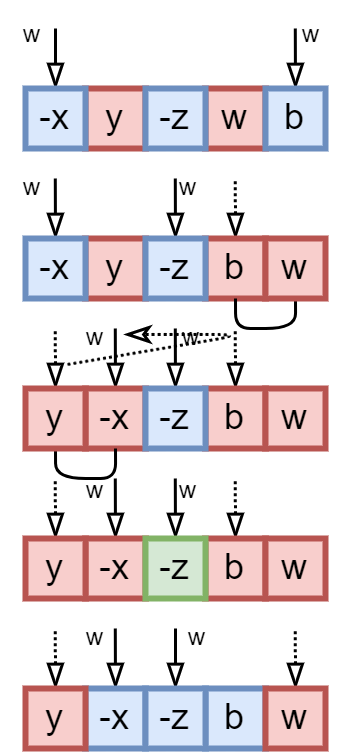
\includegraphics[width=0.4\textwidth]{figures/watched literals sifting.png}
            \caption{Пример использования для $\{\overline{x},y,\overline{z},w,b\}$, последовательность присваиваний $y \rightarrow 0$, $w \rightarrow 0$, $b \rightarrow 0$, $\overline{x} \rightarrow 0$, $\overline{z} \rightarrow 1$}
        \end{figure}
    \end{minipage}
\end{frame}

\begin{frame}[fragile] \frametitle{3. Tries}
    \begin{minipage}[m]{0.5\linewidth}
        \begin{itemize}
            \item \textbf{Идея}: использовать \textbf{trie} или префиксное дерево для представления формулы
            \item \textbf{Структура}:
            \begin{itemize}
                \item Узел дерева nil
                \item Улез дерева $\Box$
                \item Узел дерева $\langle v, pos, neg, rest \rangle$
                \item Путь от вершины до $\Box$ задает кляузу
            \end{itemize}
            \item \textbf{Интерпретация}:
            \begin{itemize}
                \item Формула $S = P \cup N \cup R$
                \item $P = \{v \cup P_1, ..., v \cup P_n\}$
                \item $N = \{\overline{v} \cup N_1, ..., \overline{v} \cup N _m\}$
                \item $R = \{R_1, ..., R_l\}$
            \end{itemize}
        \end{itemize}
    \end{minipage}\hfill
    \begin{minipage}[m]{0.45\linewidth}
        \begin{figure}
            \centering
            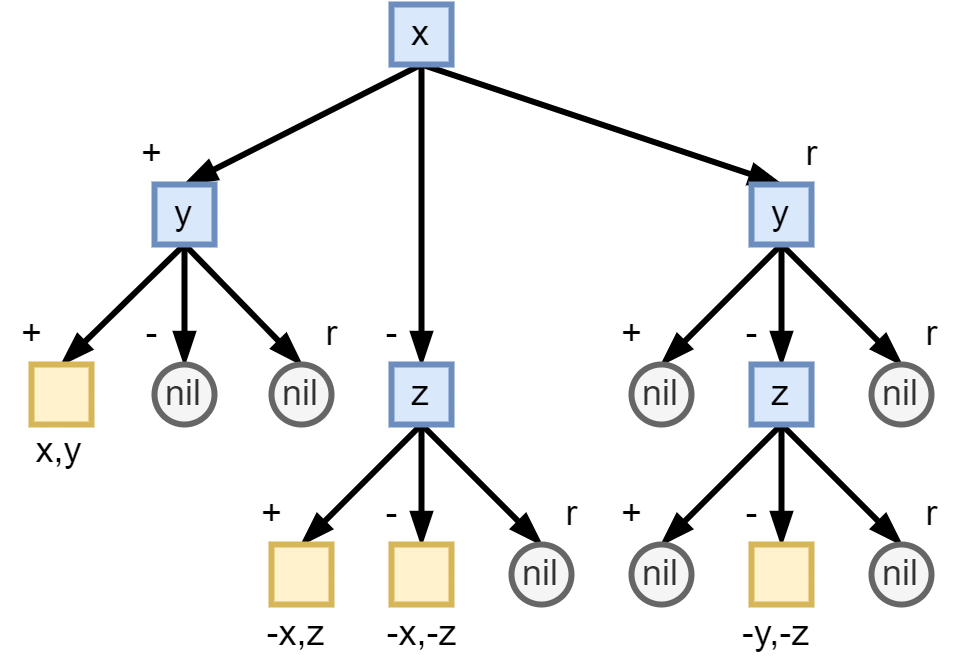
\includegraphics[width=0.9\textwidth]{figures/trie.png}
            \caption{Пример дерева для формулы $\{x,y\},\{\overline{x},z\},\{\overline{x},\overline{z}\},\{\overline{y},\overline{z}\}$}
        \end{figure}
    \end{minipage}
\end{frame}

\begin{frame}[fragile] \frametitle{4. Детали реализации (1)}
    \begin{minipage}[m]{0.5\linewidth}
        \begin{itemize}
            \item \textbf{Гибридный подход}: adjacency lists, counters, assigned literal и satisfied clause* hiding
            \item Каждый литерал дополнительно хранит список позиций, на которых он встречается в каждой кляузе
            \item Использование бит-вектора для literal hiding
            \item Максимальный размер кляузы 32 литерала $\{a,b\} \rightarrow \{a,u\},\{\overline{u},b\}$
        \end{itemize}
    \end{minipage}\hfill
    \begin{minipage}[m]{0.45\linewidth}
        \begin{figure}
            \centering
            \begin{subfigure}[b]{0.49\textwidth}
                \centering
                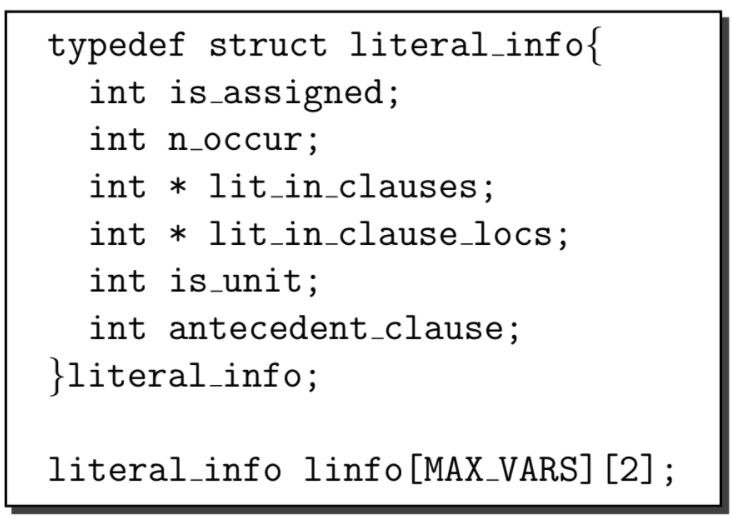
\includegraphics[width=0.95\textwidth]{figures/structure literal.png}
            \end{subfigure}
            \hfill
            \begin{subfigure}[b]{0.49\textwidth}
                \centering
                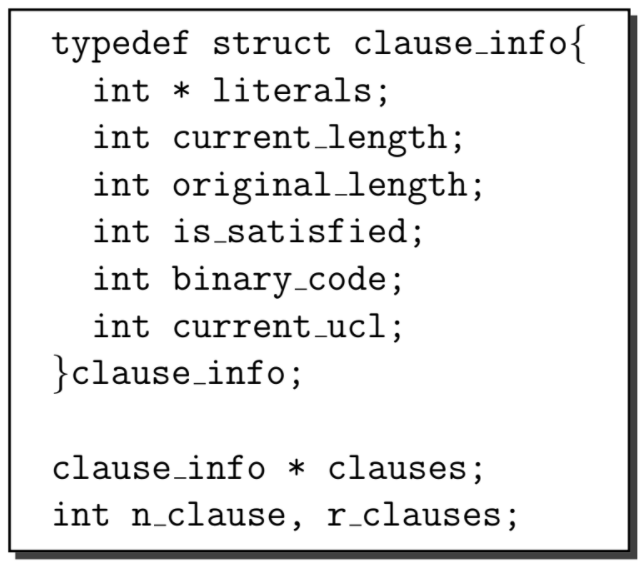
\includegraphics[width=0.95\textwidth]{figures/structure clause.png}
            \end{subfigure}
            \caption{Cтруктуры для описания информации о литералах и кляузах (изображения из работы [6])}
        \end{figure}
    \end{minipage}
\end{frame}

\begin{frame}[fragile] \frametitle{4. Детали реализации (2)}
    \begin{minipage}[m]{0.5\linewidth}
        \begin{itemize}
            \item Информация о выполненых кляузах и о тех, в которых вычеркнули литерал
            \item Для каждого уровня присваивания литералу значения --- количесвто выполненых кляуз и тех, из которых вычеркнули литерал
            \item Используется для \textbf{backtracking}
            \item Для каждой переменной информация о присваивании значения
            \item Используется для \textbf{non-chronological backtracking} и обратного bfs-обхода для \textbf{clause learning}
        \end{itemize}
    \end{minipage}\hfill
    \begin{minipage}[m]{0.45\linewidth}
        \begin{figure}
            \centering
            \begin{subfigure}[b]{0.49\textwidth}
                \centering
                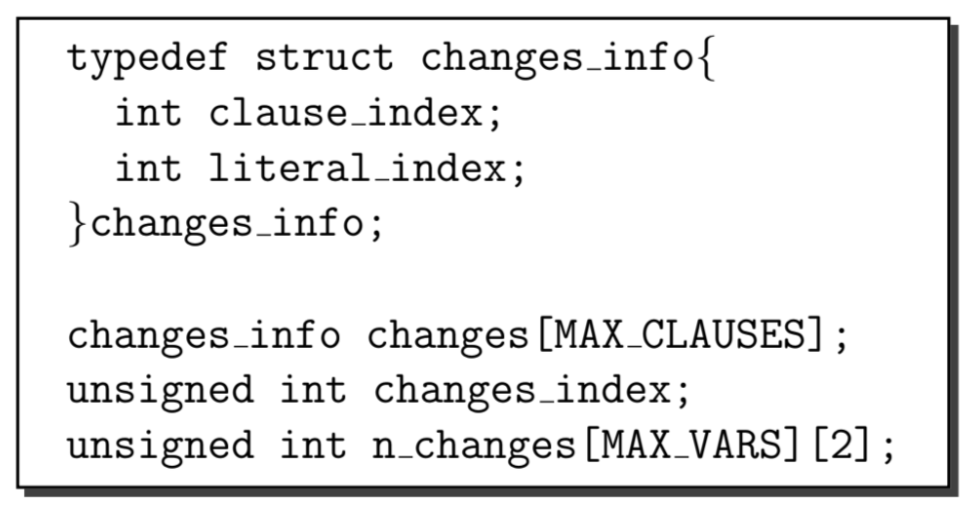
\includegraphics[width=0.95\textwidth]{figures/structure changes.png}
            \end{subfigure}
            \hfill
            \begin{subfigure}[b]{0.49\textwidth}
                \centering
                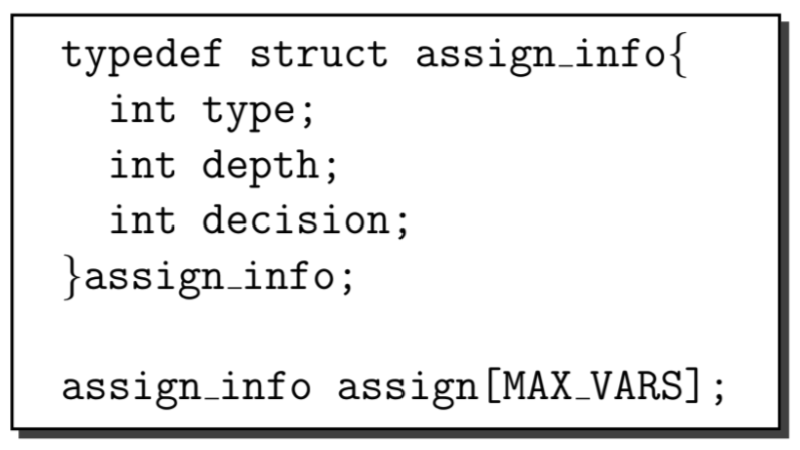
\includegraphics[width=0.95\textwidth]{figures/structure assign info.png}
            \end{subfigure}
            \caption{Cтруктуры для описания стека изменений и информации о присваиваниях значений (изображения из работы [6])}
        \end{figure}
    \end{minipage}
\end{frame}

\begin{frame}[fragile] \frametitle{Матералы презентации}
    \begin{itemize}
        \item[1] Zhang, Hansong and Mark E. Stickel. (1994). “Implementing the Davis-Putnam Algorithm by Tries.” Journal of Automated Reasoning
        \item[2] João P. Marques Silva and Karem A. Sakallah. (1997). GRASP — a new search algorithm for satisfiability. In Proceedings of the 1996 IEEE/ACM international conference on Computer-aided design (ICCAD '96). IEEE Computer Society, USA, 220–227.
        \item[3] Lintao Zhang and Sharad Malik. 2002. The Quest for Efficient Boolean Satisfiability Solvers. In "Proceedings of the 14th International Conference on Computer Aided Verification". Springer-Verlag, Berlin, Heidelberg, 17–36.
        \item[4] Lynce, I. and Marques-silva, J.. (2002). Efficient Data Structures for Fast SAT Solvers. 
        \item[5] Eén, N. and Sörensson, N. (2003). An Extensible SAT-solver. SAT.
        \item[6] Ahmed, T. (2009). An Implementation of the DPLL Algorithm.
    \end{itemize}
\end{frame}

\end{document}
